\documentclass{standalone}
\standaloneconfig{border=2mm 2mm 2mm 2mm}
\usepackage{tikz}
\usetikzlibrary{calc} 
\begin{document}

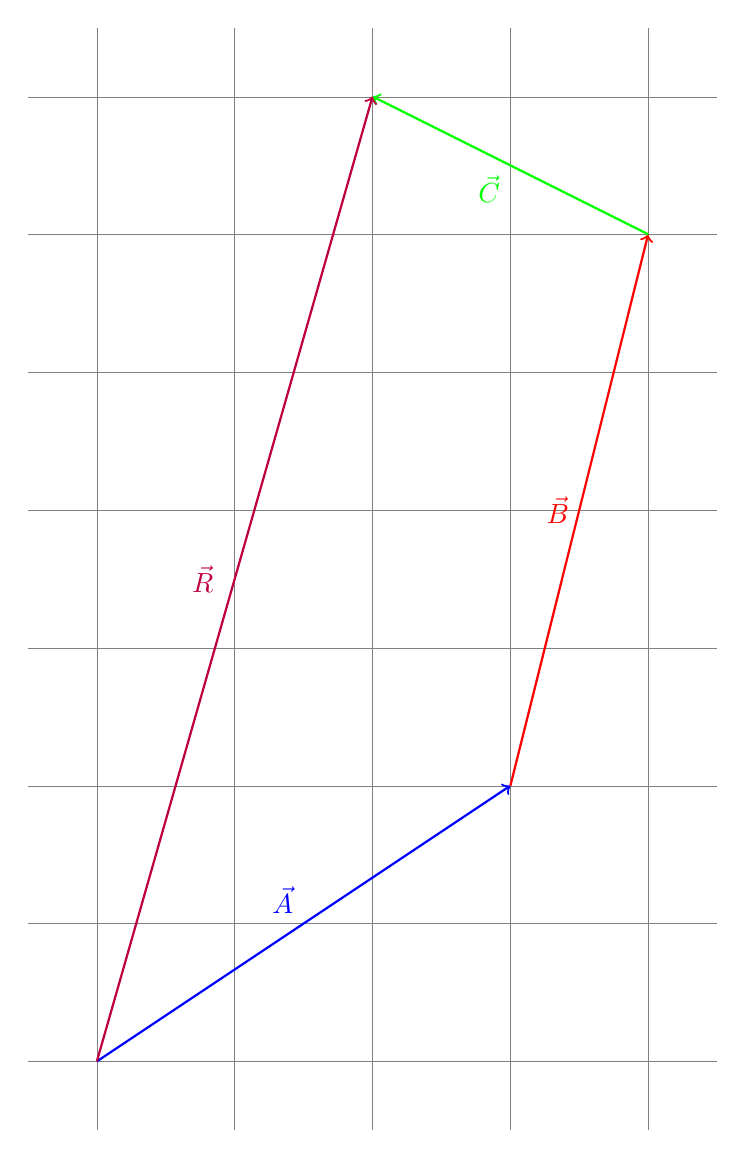
\begin{tikzpicture}[scale=1.75]
    \draw [help lines] (-.5,-0.5) grid (4.5,7.5);

    % Three vectors, A, B, and C, and their resultant, R.
    % Define the origin
    \coordinate (O) at (0,0);
    
    % Define vectors A, B, and C by their terminal points
    \coordinate (A) at (3,2);    % Vector A from (0,0) to (3,2)
    \coordinate (B) at (1,4);    % Vector B from (0,0) to (1,4)
    \coordinate (C) at (-2,1);   % Vector C from (0,0) to (-2,1)
    
    % Calculate the resultant R as the sum of A, B, and C
    \coordinate (R) at ($(A) + (B) + (C)$);
    
    % Draw vectors A, B, C from the origin
    \draw[->, thick, blue] (O) -- (A) node[midway, above left] {$\vec{A}$} coordinate (A');
    \draw[->, thick, red] (A') -- ($(A) + (B)$) node[midway, left] {$\vec{B}$} coordinate (B');
    \draw[->, thick, green] (B') -- ($(B') + (C)$) node[midway, below left] {$\vec{C}$};
    
    % Draw the resultant vector R from the origin
    \draw[->, thick, purple] (O) -- (R) node[midway, left=4pt] {$\vec{R}$};

\end{tikzpicture}

\end{document}
